\title {\ZHH \huge 从手机到internet}
\author {\ENL \Hfive \href{www.gaccob.com}}

\begin {document}

\maketitle

% section 1
\section {\ZHH 手机到internet之间的数据传输} {
    \begin {figure} [htbp]
        \centering
        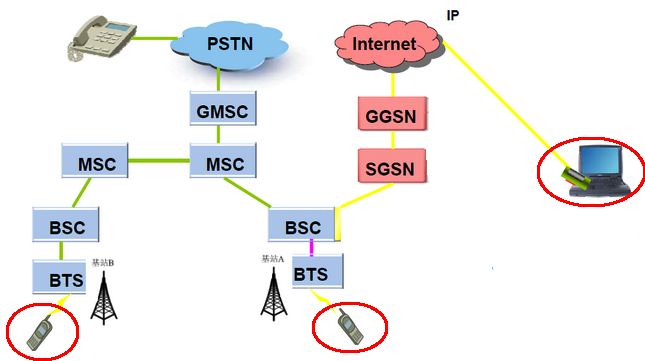
\includegraphics [width=400pt, keepaspectratio] {transfer.png}
    \end {figure}

    {\ZHH 详细解释一下相关术语: }

    \begin {itemize}
        \item { \textcolor {blue} {基站收发台BTS(Base Transceiver Station) } } \\
        { 由BSC控制, 服务于某个小区的无线收发信设备, 完成BSC与无线信道之间的转换, 实现BTS和移动台之间通过空中接口的无线传输及相关的控制功能. } \\
        { BTS和移动终端(专业术语叫做移动台, MS)之间的是\textcolor{blue}{Um接口}, 也称空中接口, 在GSM/GPRS/EDGE网络中, 传输MS与网络之间的信令信息和业务信息. } \\

        \item { \textcolor {blue} {基站控制器BSC(Base Station Control)} } \\
        { BSC在基站子系统中起控制器和话务集中器作用, 一个基站控制器根据话务量可以控制数十个BTS. } \\
        { BTS和BSC之间是\textcolor{blue}{Abis接口}: 遵循GSM规范08.5X系列要求, 在Abis接口上BSC提供BTS配置, BTS监测, BTS测试及业务控制等信令控制信息. } \\

        \item { \textcolor {blue} {基站子系统BSS} } \\
        { 可以由一个BSC和多个BTS组成, BSC根据业务量, 可以控制多个BTS. BTS负责传输, BSC负责管理和控制. } \\

    \end {itemize}
}

\end {document}
